\chapter{Implementierung}

Es sollen nun einige Beispiele aus der entstandenen Applikation gezeigt werden. Eine vollständige Anleitung kann einem separaten Dokument entnommen werden

\section{Weekly Standup}

Ein  Nutzer des Weekly Standup Plugins würde auf der entsprechenden Seite für sein Team folgendes sehen:

\begin{figure}[H]
	\centering
	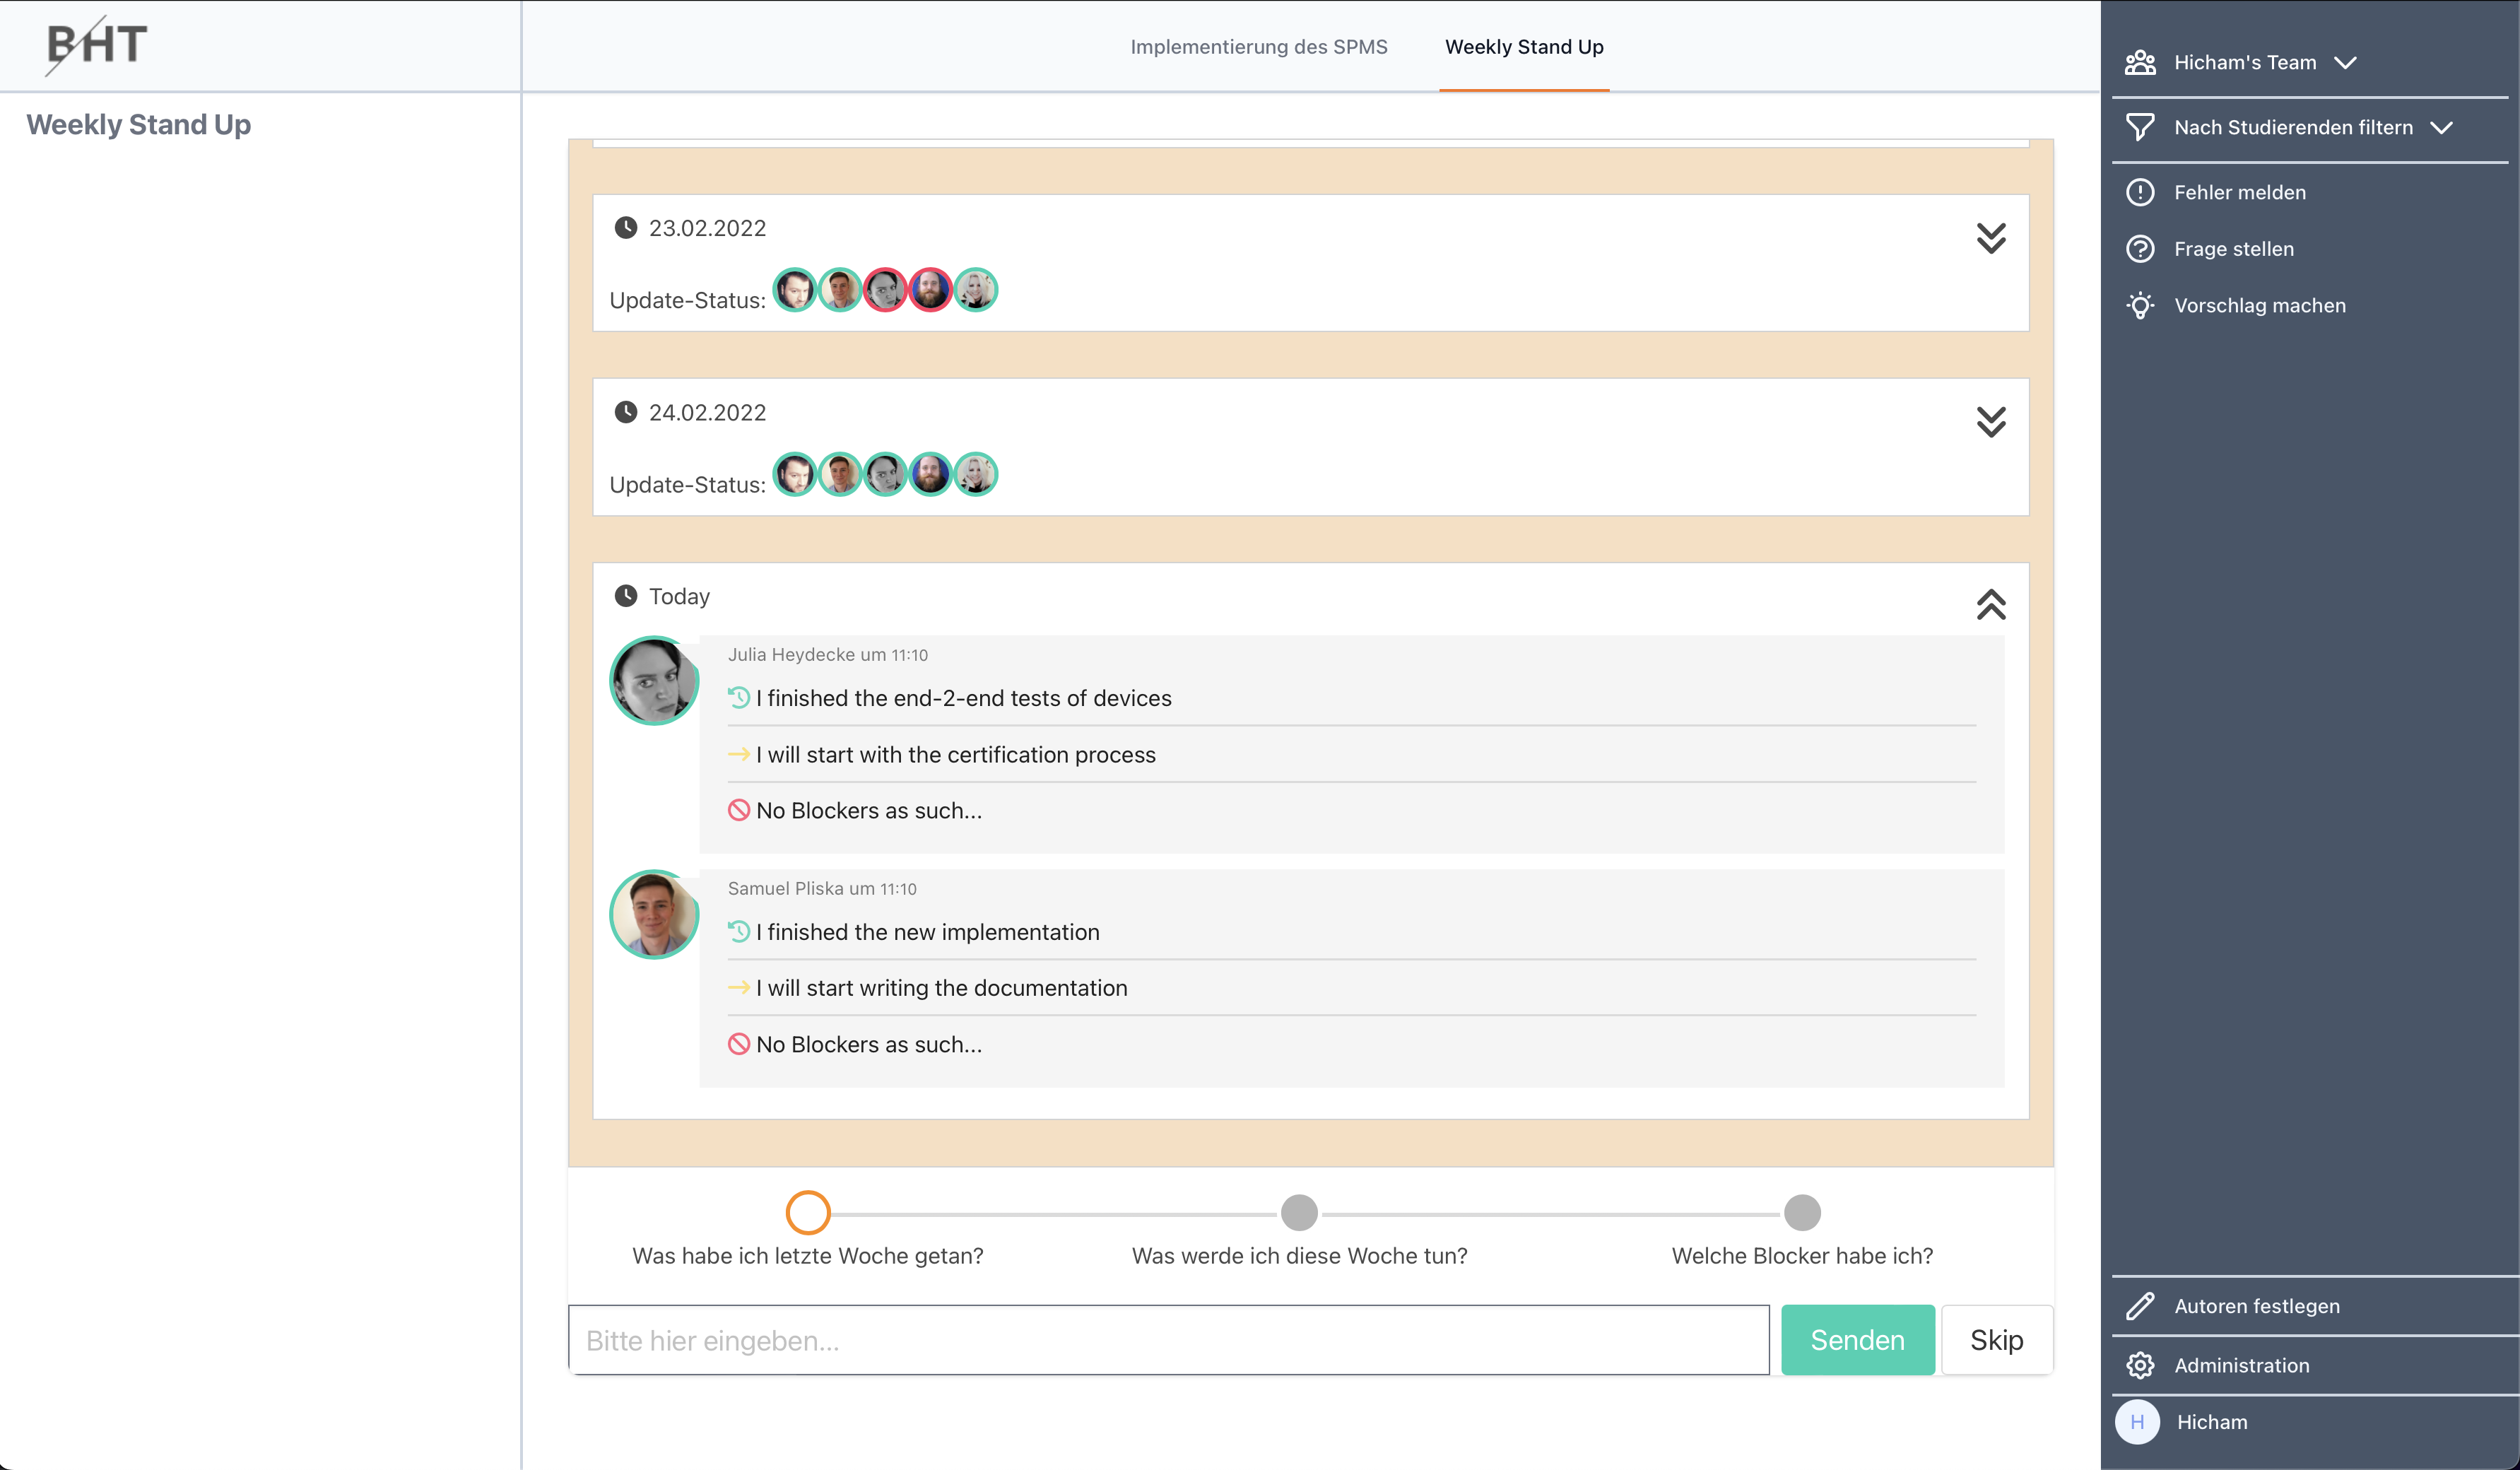
\includegraphics[width=0.95\textwidth]{impl-overview.png}
    \caption{Nutzeransicht}
	\label{fig:userview}
\end{figure}

In dieser Ansicht kann sich ein Nutzer über Vergangene Meetings verschaffen oder für das nächste Meeting sein Feedback abgegeben.

\section{Kartenansicht}

Alle Meetings werden auf sog. Karten dargestellt. Diese Karten können zwei Zustände annehmen: 
\begin{figure}[H]
	\centering
	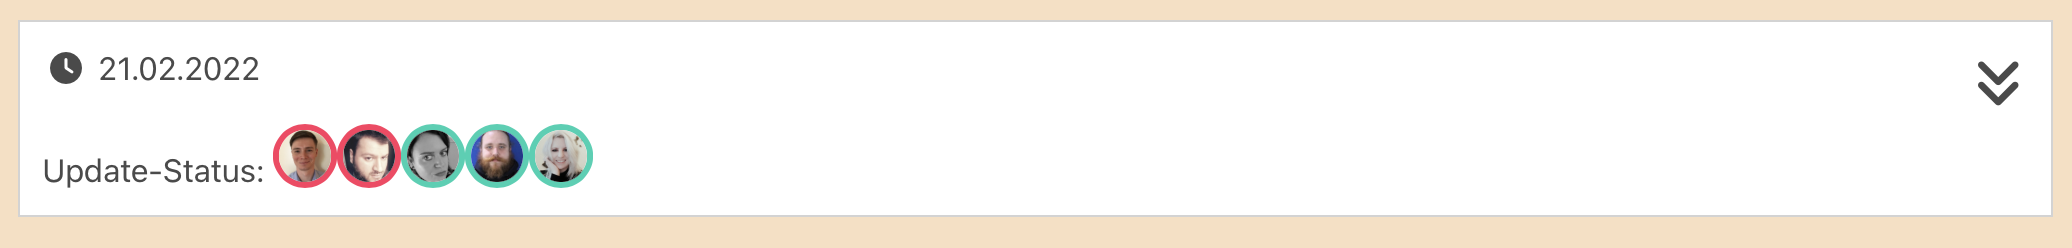
\includegraphics[width=0.95\textwidth]{impl-card1.png}
    \caption{Zusammengeklappte Karte}
	\label{fig:collapsedCard}
\end{figure}

Einen kollabierten Zustand, auf dem nur die wichtigsten Informationen zu sehen sind. Oben links das Datum zu dem das Meeting terminiert war und Darunter die Eingeladenen Teilnehmer.
Die Umrandung der Avatare Der Teilnehmer gibt hierbei ob ein Teilnehmer für dieses Meeting ein Feedback eingereicht hat oder nicht. 
\begin{itemize}
\item \textbf{Grün:} Der Teilnehmer hat teilgenommen
\item \textbf{Rot:} Der Teilnehmer hat \textbf{\textul{nicht}}teilgenommen
\end{itemize}
Dies ist der standardmäßige Zustand für vergangene Meetings. Das aktuelle Meeting wird in einer ausführlicheren Form dargestellt:

\begin{figure}[H]
	\centering
	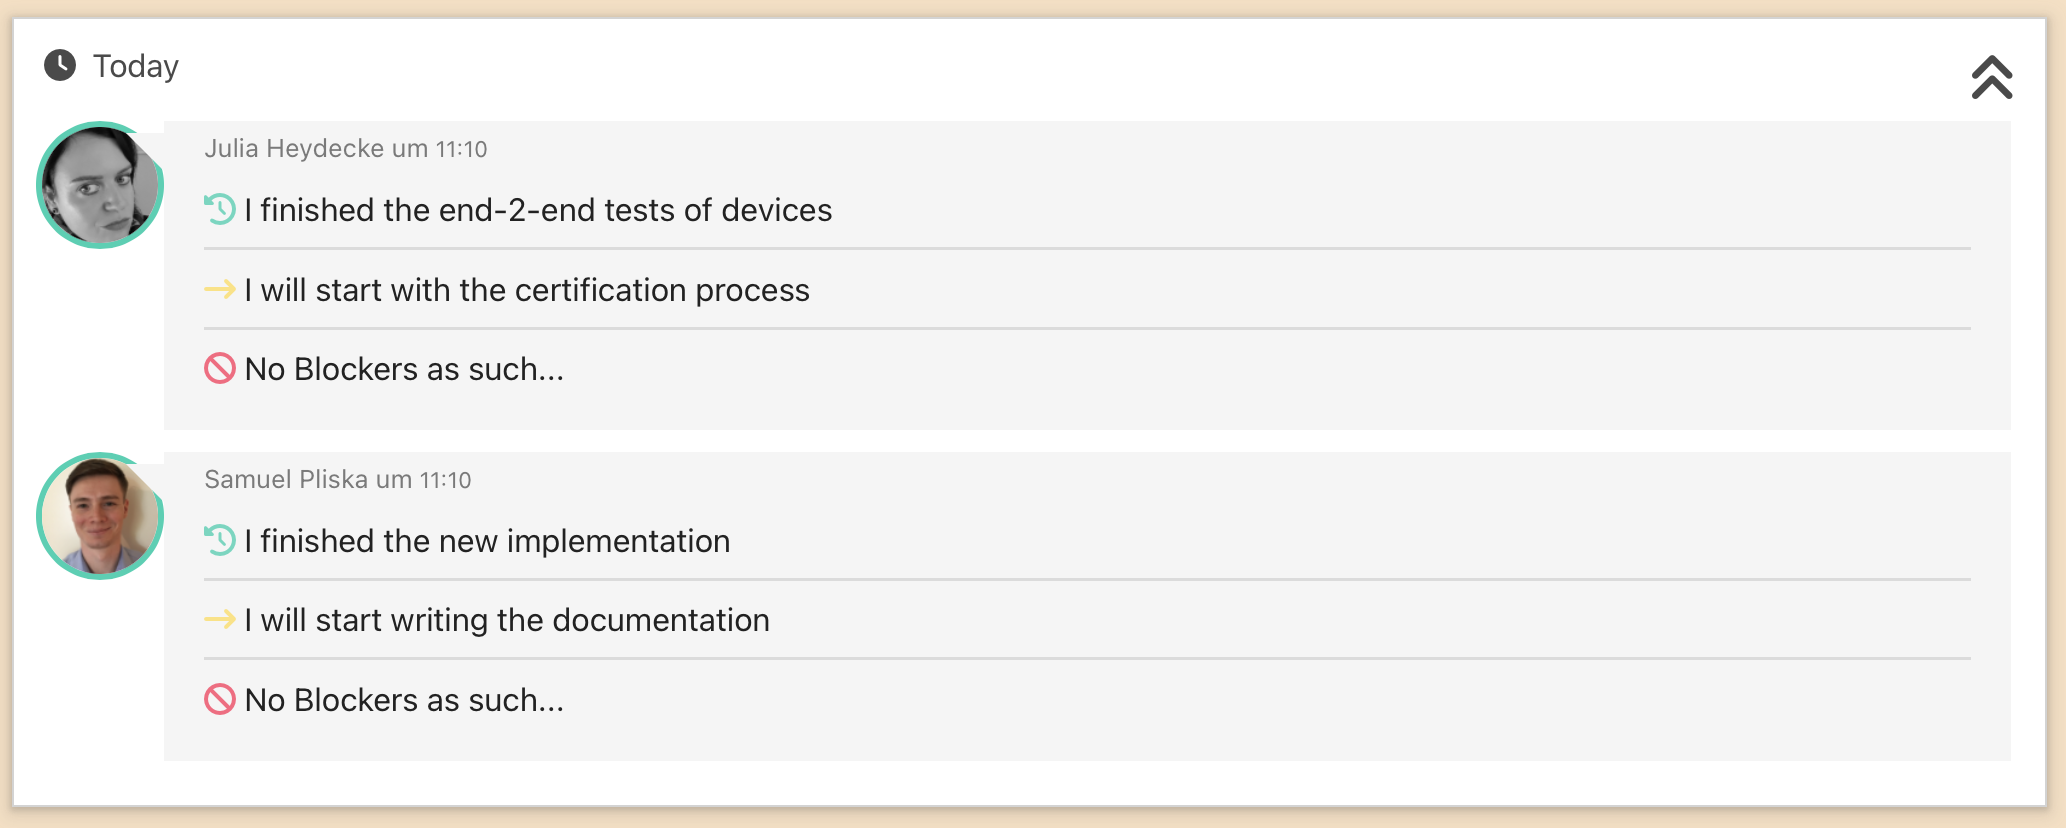
\includegraphics[width=0.95\textwidth]{impl-card2.png}
    \caption{Vollständige Kartenansicht}
	\label{fig:uncollapsedCard}
\end{figure}

Auf einer Karte werden jeweils die Teilnehmer mit ihren Antworten auf die Fragen angezeigt.

Ein wechsel zwischen diesen zuständen wird mittels des Doppelchevrons an der oberen rechten Ecke durchgeführt.

\section{Eingabewizzard}

Die Eingabe des Feedbacks für das Weekly Standup erfolgt durch eine Textbox am unteren Rand des Blocks.

Hierbei wird dem Nutzer zu jeder Zeit angezeigt was er schon abgegeben hat und was von ihm noch erwartet wird.

\begin{figure}[H]
	\centering
	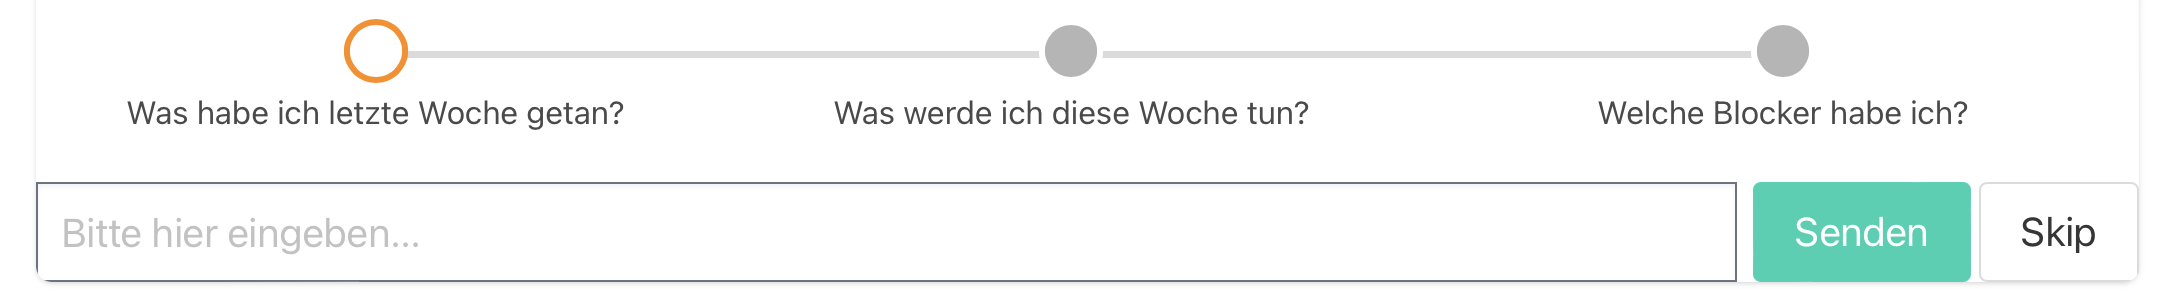
\includegraphics[width=0.95\textwidth]{impl-wiz1.png}
    \caption{Feedback: Schritt 1 von 3}
	\label{fig:wizzard1}
\end{figure}

Durch Senden oder Skippen der Antwort gelangt der User zum nächsten Schritt.

\begin{figure}[H]
	\centering
	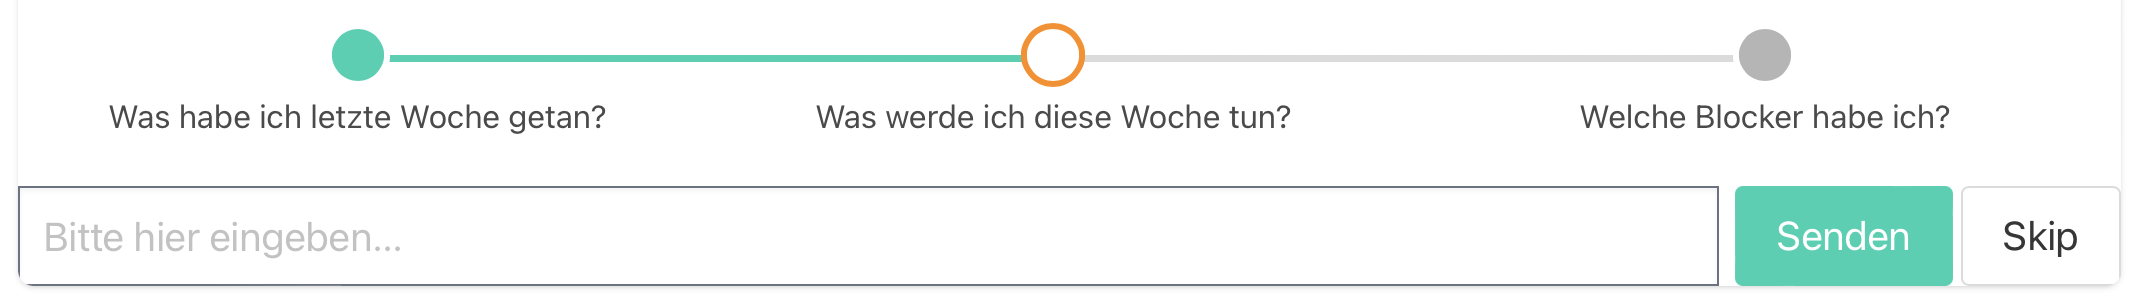
\includegraphics[width=0.95\textwidth]{impl-wiz2.png}
    \caption{Feedback: Schritt 2 von 3}
	\label{fig:wizzard2}
\end{figure}

Bei Betätigung des Skip Buttons wird das Feedback des Users durch eine Standardantwort erfasst. Dies dient dazu, damit haben die Nutzer die Möglichkeit ein Feedback abzugeben, auch wenn nichts passiert ist und werden somit nicht als abwesend erfasst (Ein möglicher Use Case wäre die Antwort auf die Frage nach der letzten Woche in der ersten Projekt Woche).

Eine mögliche Verbesserung hier wäre es, Nutzern vorgefertigte Antworten anzubieten, gerade wenn sie noch nie mit Weekly Standups gearbeitet haben

\section{Administrative Ansicht}

Ein Dozent oder anderer User der einen Kurs anlegt, kann beim anlegen eines Kurses das Plugin als ein Block dem \ac{SPMS} hinzufügen.\\

\begin{figure}[H]
	\centering
	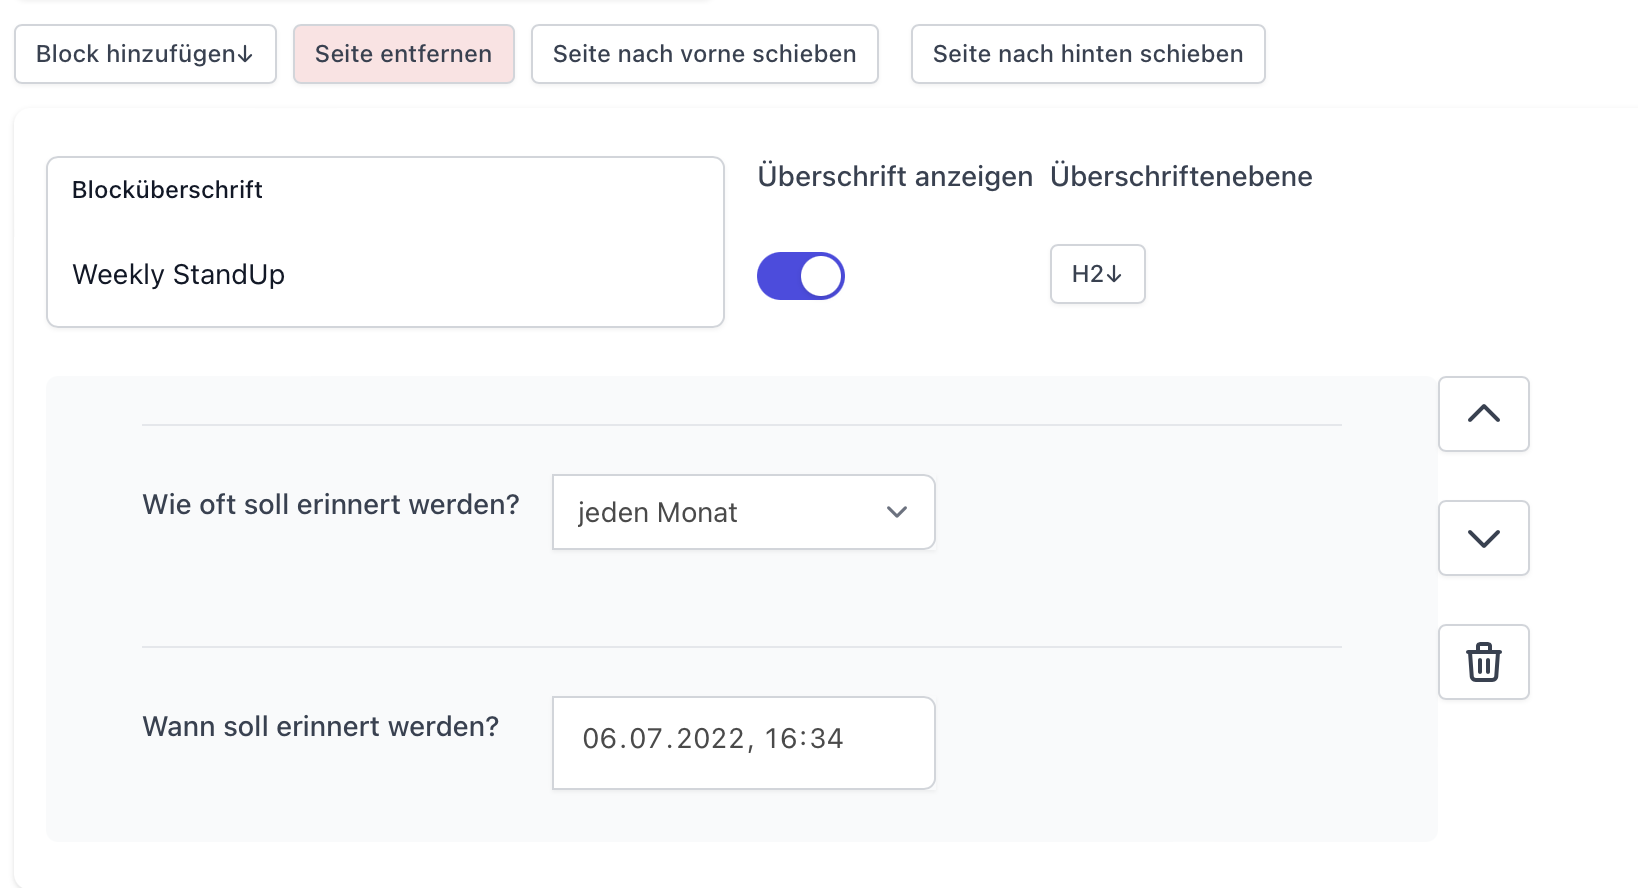
\includegraphics[width=0.95\textwidth]{impl-admin.png}
    \caption{Ansicht beim einrichten des Weekly Standup Plugins}
	\label{fig:adminpanel}
\end{figure}

Für den Block bestehen folgende Einstellungsmöglichkeiten:

\begin{itemize}
    \item \textbf{Überschrift:} Gibt dem Block eine Überschrift, bei bedarf kann diese auch Abgeschaltet werden oder als eine andere Ebene dargestelt werden (Standardmäßig ist die \verb|<h2 />| Ebene vorgesehen) 
    \item \textbf{Häufigkeit:} Gibt an wie häufig das Standup Meeting einen neuen Zyklus beginnt. Derzeit gibt es folgende Möglichkeiten:
    \begin{itemize}
        \item Wöchentlich
        \item Monatlich
      \end{itemize}
    \item \textbf{Erinnerung:} Gibt an ab wann eine Erinnerung verschickt werden soll. Dies legt intern einen Task an welcher mit dem zuvor gewählten Intervall ausgeführt wird
\end{itemize}
